\documentclass[11pt,a4paper]{article}
\usepackage[utf8]{inputenc}
\usepackage[T1]{fontenc}
\usepackage{tgpagella}
\usepackage[spanish]{babel}
\usepackage{geometry}
\usepackage{booktabs}
\usepackage{xcolor}
\usepackage{titlesec}
\usepackage{fancyhdr}
\usepackage[parfill]{parskip}
\usepackage[expansion=false]{microtype}
\usepackage{hyperref}
\usepackage{setspace}
\usepackage{graphicx}
\usepackage{needspace}

\widowpenalty=10000
\clubpenalty=10000
\displaywidowpenalty=10000

\geometry{top=3.0cm,bottom=3.0cm,left=3.5cm,right=3.5cm}
\setlength{\parskip}{0.65em}
\setlength{\parindent}{0em}

\definecolor{azulai}{RGB}{30,80,140}
\definecolor{doradoai}{RGB}{140,90,0}
\definecolor{grisai}{RGB}{70,70,70}

\titleformat{\section}{\Large\bfseries\color{azulai}}{}{0em}{}[{\color{azulai}\titlerule[0.5pt]}]
\titlespacing*{\section}{0pt}{1.4em}{0.5em}

\titleformat{\subsection}{\large\bfseries\color{doradoai}}{}{0em}{}
\titlespacing*{\subsection}{0pt}{1.0em}{0.35em}

\titleformat{\subsubsection}{\normalsize\bfseries\color{grisai}}{}{0em}{}
\titlespacing*{\subsubsection}{0pt}{0.7em}{0.25em}

\pagestyle{fancy}\fancyhf{}
\rhead{\textcolor{grisai}{\small Amaya Beatriz — Arquitectura Interna}}
\lhead{\textcolor{grisai}{\small Plutón · Casa 8 · Casa 12 · Quirón · Lilith}}
\cfoot{\textcolor{grisai}{\small\thepage}}
\renewcommand{\headrulewidth}{0.3pt}

\hypersetup{colorlinks=true,linkcolor=azulai,urlcolor=azulai}
\setstretch{1.25}
\tolerance=1500
\emergencystretch=4em

\begin{document}

\begin{titlepage}
  \centering
  \vspace*{1.5cm}
  {\Huge\bfseries\color{azulai} Plutón · Casa 8 · Casa 12}\\[0.35cm]
  {\Huge\bfseries\color{azulai} Quirón · Lilith}\\[0.5cm]
  {\large\color{grisai} Arquitectura Interna}\\[0.3cm]
  {\small\itshape\color{grisai} Sombra, herida, intimidad y profundidad psíquica}\\[2cm]
  {\huge\color{doradoai} Amaya Beatriz}\\[1.5cm]
  {\Large 30/10/1976 \quad 22:10}\\[0.3cm]
  {\Large Zaragoza, España}\\[0.3cm]
  {\normalsize Lat: 41.6916° \quad Lon: -0.9101° \quad UTC+01:00}\\[0.3cm]
  {\normalsize Ascendente: Cáncer 16°08' \quad
    MC: Piscis 25°32'}\\[2cm]

  \begin{tabular}{ll}
    \textbf{Plutón:}  & Libra — Casa 4 12°36' \\
    \textbf{Quirón:}  & Aries — Casa 10 29°12' (retrógrado) \\
    \textbf{Lilith:}  & Tauro — Casa 11 10°34' \\
    \textbf{Casa 8:}  & Acuario \\
    \textbf{Casa 12:} & Géminis \\
  \end{tabular}\\[2cm]

  \vfill
  {\small Generado el 20/05/2026}
\end{titlepage}

\tableofcontents
\newpage

\section{Datos de referencia}

\begin{center}
\begin{tabular}{llll}
  \toprule
  \textbf{Punto} & \textbf{Signo} & \textbf{Casa} & \textbf{Posición} \\
  \midrule
  Plutón & Libra & 4 & 12°36' \\
  Quirón (retrógrado) & Aries & 10 & 29°12' \\
  Lilith          & Tauro & 11 & 10°34' \\
  Casa 8          & Acuario             & ---                  & --- \\
  Casa 12         & Géminis            & ---                  & --- \\
  Ascendente      & Cáncer         & ---                  & 16°08' \\
  Medio Cielo     & Piscis          & ---                  & 25°32' \\
  \bottomrule
\end{tabular}
\end{center}

\vspace{0.5cm}
\textbf{Aspectos relevantes:}

\begin{center}
\begin{tabular}{lllll}
  \toprule
  \textbf{Punto 1} & \textbf{Asp.} & \textbf{Punto 2} & \textbf{Aspecto} & \textbf{Orbe} \\
  \midrule
  Plutón & sex & Neptuno & Sextil & 0.2° \\
  Plutón & sex & Venus & Sextil & 0.2° \\
  Plutón & sex & Saturno & Sextil & 3.6° \\
  Plutón & tri & Luna & Trígono & 6.5° \\
  Quirón & opo & Mercurio & Oposición & 3.6° \\
  Quirón & conj & Nodo Sur & Conjunción & 4.3° \\
  Lilith & opo & Sol & Oposición & 3.0° \\
  \bottomrule
\end{tabular}
\end{center}

\begin{center}
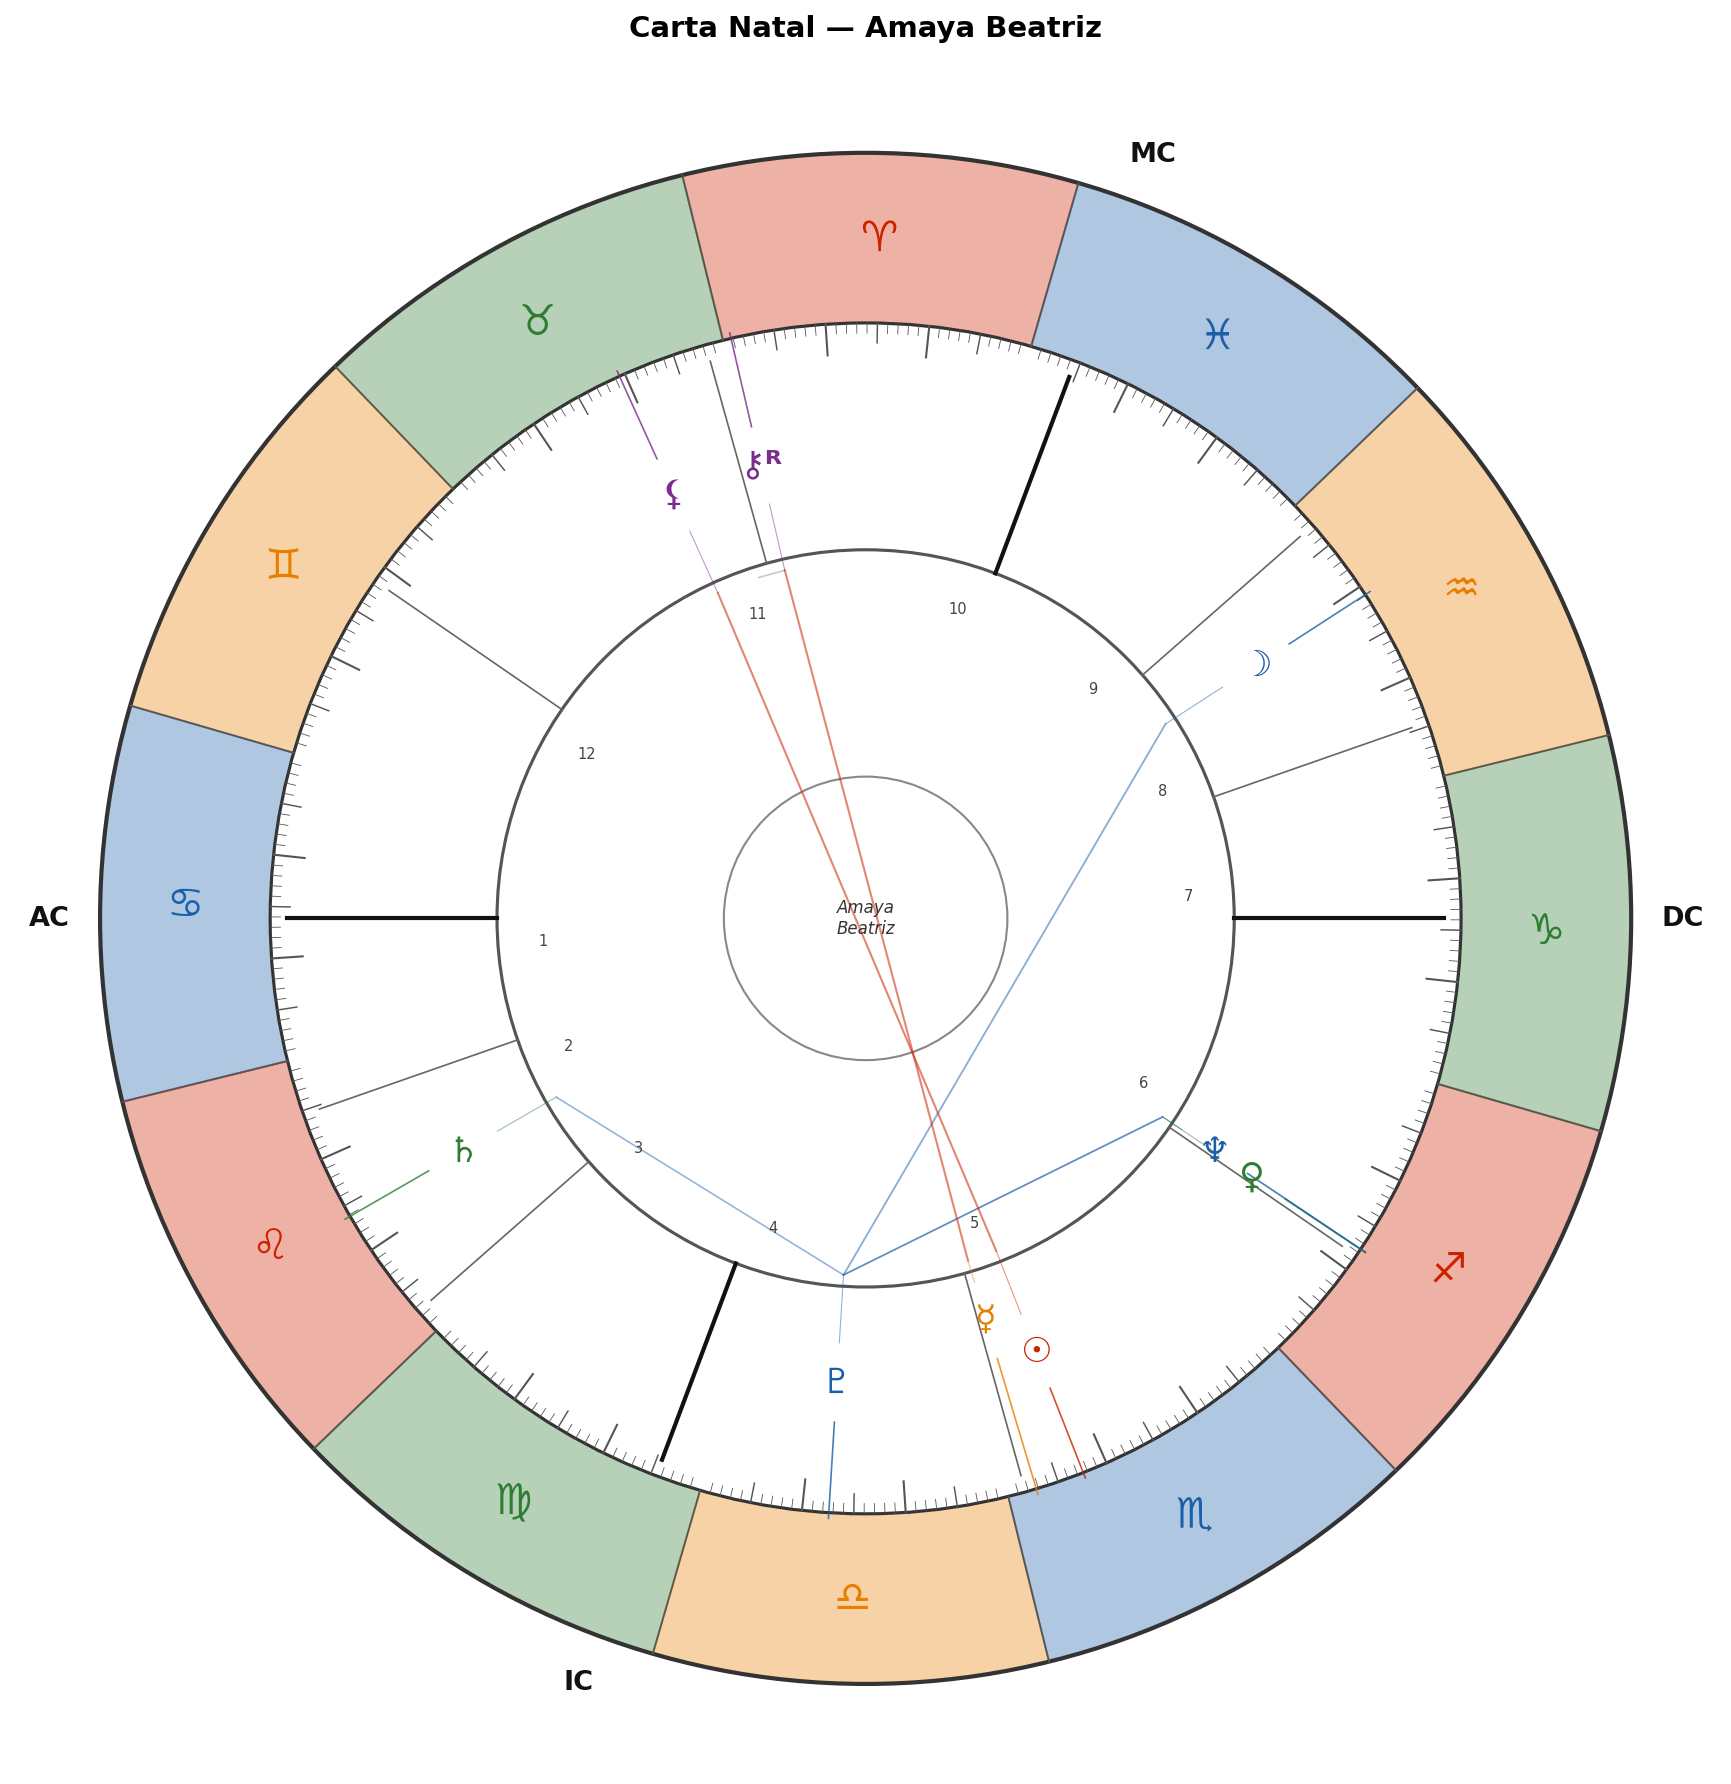
\includegraphics[width=0.72\textwidth]{Amaya_Beatriz_rueda.png}
\end{center}

\Needspace{3\baselineskip}

\section{Interpretación}

\begin{center}
{\small\itshape
Este documento no busca definirte. Se acerca a zonas donde pueden aparecer intensidad,\\
defensa, herida, vulnerabilidad, deseo, retiro o dificultad para poner en palabras lo que ocurre.
}
\end{center}

\vspace{0.8cm}

\Needspace{10\baselineskip}
\vspace{0.4cm}

\subsection{1. Marco general}

Este documento entra en zonas de la carta que suelen vivirse con más intensidad, más defensa o más dificultad para nombrar. No describe una identidad fija ni una condena personal. Se acerca a lugares donde pueden aparecer miedo, control, vergüenza, deseo, aislamiento, dependencia, heridas antiguas o reacciones difíciles de comprender desde fuera.

Plutón en Libra, Casa 4: muestra dónde puedes vivir procesos intensos de transformación, pérdida de control, apego, defensa o profundidad emocional.
Quirón en Aries, Casa 10: muestra una zona especialmente sensible, donde puede haber herida, inseguridad, vergüenza o necesidad de protección.
Lilith en Tauro, Casa 11: muestra una parte de ti menos domesticable, más instintiva, que puede reaccionar con fuerza cuando se siente atrapada, reducida o invadida.

La Casa 8 en Acuario habla de cómo atraviesas la vulnerabilidad, la intimidad, la pérdida, la confianza y los vínculos que remueven profundamente.
La Casa 12 en Géminis habla de cómo vives el retiro, la sensibilidad, el agotamiento emocional, lo inconsciente y aquello que cuesta poner en palabras.

Aspectos principales observados en este bloque: Plutón–Neptuno en sextil (orbe 0.19°), Plutón–Venus en sextil (orbe 0.23°), Plutón–Saturno en sextil (orbe 3.57°), Plutón–Luna en trígono (orbe 6.49°), Quirón–Mercurio en oposición (orbe 3.59°), Quirón–Nodo Sur en conjunción (orbe 4.34°), Lilith–Sol en oposición (orbe 2.98°).

\Needspace{10\baselineskip}
\vspace{0.4cm}

\subsection{2. Plutón — Intensidad, control y transformación}

\Needspace{6\baselineskip}
\subsubsection*{Plutón en Libra — Casa 4}

Plutón en Libra muestra una intensidad profunda ligada al vínculo, el deseo, la dependencia, la comparación y el miedo al conflicto. Las relaciones pueden tocar zonas muy hondas de ti, especialmente cuando aparece la posibilidad de pérdida, rechazo o desequilibrio.

La sombra puede aparecer como complacencia, manipulación sutil, dependencia afectiva o necesidad de controlar la armonía para no sentir amenaza. A veces puedes ceder demasiado y luego resentirte por dentro.

La transformación pasa por mirar qué parte de ti negocia su verdad para no perder vínculo. Tu poder crece cuando puedes amar, elegir y relacionarte sin abandonar tu centro.

Plutón en casa 4 muestra procesos profundos ligados a la infancia, la familia, el hogar y la sensación de pertenencia. Puede haber memorias emocionales intensas o ambientes familiares donde ciertas cosas no podían hablarse claramente.

A veces existe necesidad de controlar mucho el espacio personal porque el cuerpo no termina de relajarse del todo. También puede aparecer miedo a depender emocionalmente o dificultad para sentir verdadera seguridad interna.

La transformación pasa por revisar qué parte de tu vida sigue organizada alrededor de heridas antiguas. Construir hogar deja de ser protegerte de todo y empieza a ser poder descansar.

Plutón–Neptuno en sextil (orbe 0.19°).
Plutón en aspecto con Neptuno intensifica la sensibilidad, la percepción profunda y la relación con lo invisible o difícil de explicar. Puede haber mucha permeabilidad emocional, intuición o dificultad para distinguir entre deseo, miedo y fantasía.

A veces necesitas poner límites claros a lo que absorbes o idealizas.

El sextil abre una posibilidad de aprendizaje consciente. Puede no activarse solo, pero cuando le prestas atención permite trabajar esta combinación de una forma más manejable.

Este aspecto es muy cerrado, por lo que suele sentirse con bastante fuerza. No aparece como algo lejano o secundario, sino como una dinámica que puede activarse con claridad en momentos importantes.

Plutón–Venus en sextil (orbe 0.23°).
Plutón en aspecto con Venus intensifica mucho el amor, el deseo, el apego y la manera en que te vinculas. Las relaciones pueden remover zonas profundas de vulnerabilidad, miedo a la pérdida o necesidad de control.

A veces lo afectivo se vive con mucha intensidad, incluso cuando intentas mantenerlo ligero.

El sextil abre una posibilidad de aprendizaje consciente. Puede no activarse solo, pero cuando le prestas atención permite trabajar esta combinación de una forma más manejable.

Este aspecto es muy cerrado, por lo que suele sentirse con bastante fuerza. No aparece como algo lejano o secundario, sino como una dinámica que puede activarse con claridad en momentos importantes.

Plutón–Saturno en sextil (orbe 3.57°).
Plutón en aspecto con Saturno toca zonas profundas de control, miedo, responsabilidad y resistencia. Puede haber sensación de carga, dureza interna o necesidad de sostenerte incluso en situaciones muy exigentes.

A veces puedes confundir fortaleza con aguantar demasiado.

El sextil abre una posibilidad de aprendizaje consciente. Puede no activarse solo, pero cuando le prestas atención permite trabajar esta combinación de una forma más manejable.

Aunque el orbe es más amplio, el aspecto puede seguir apareciendo como un matiz importante dentro de la carta.

Plutón–Luna en trígono (orbe 6.49°).
Plutón en aspecto con la Luna intensifica mucho la vida emocional. Puede haber emociones profundas, miedo al abandono, necesidad de control afectivo o dificultad para relajarte del todo en la intimidad.

A veces sientes más de lo que muestras, o proteges mucho lo que ocurre dentro de ti.

El trígono facilita que esta combinación fluya con más naturalidad. No elimina la profundidad del aspecto, pero puede hacer que encuentres recursos internos con mayor facilidad.

Aunque el orbe es más amplio, el aspecto puede seguir apareciendo como un matiz importante dentro de la carta.

\Needspace{10\baselineskip}
\vspace{0.4cm}

\subsection{3. Quirón — Herida, sensibilidad y protección}

\Needspace{6\baselineskip}
\subsubsection*{Quirón en Aries — Casa 10 (retrógrado)}

Quirón en Aries suele mostrar una herida ligada a la afirmación personal, la iniciativa y el derecho a ocupar espacio. Puede costarte actuar con espontaneidad cuando sientes que podrías equivocarte, molestar o exponerte demasiado.

A veces aparece miedo al conflicto, inseguridad respecto a tu fuerza o sensación de tener que demostrar constantemente que puedes por ti misme. También puede existir una relación ambivalente con la rabia: contenerla demasiado o expresarla de golpe cuando ya no puedes sostenerla.

El aprendizaje pasa por permitirte existir sin tener que justificar continuamente tu presencia, tu deseo o tu manera de actuar.

Quirón en casa 10 suele mostrar heridas ligadas al reconocimiento, la autoridad y la sensación de valor frente al mundo. Puede haber mucha sensibilidad respecto al éxito, el fracaso o la percepción externa.

A veces sientes que necesitas demostrar constantemente capacidad, fortaleza o competencia para sentirte segura. También puede costarte mucho mostrar vulnerabilidad en espacios donde sientes que te observan.

El aprendizaje pasa por descubrir que tu valor no depende únicamente de lo que logras o sostienes hacia fuera.

Quirón está retrógrado. La herida tiende a vivirse de manera muy interna. Puede costarte mostrar con claridad dónde duele, incluso cuando esa sensibilidad está muy presente. A veces aprendes a protegerte antes de entender del todo qué parte de ti necesitaba cuidado.

Quirón–Mercurio en oposición (orbe 3.59°).
Quirón en aspecto con Mercurio toca la voz, la palabra y la confianza en tu manera de pensar. Puede haber miedo a expresarte mal, a que no te entiendan o a que lo que dices no tenga valor.

A veces la herida aparece en forma de duda constante sobre tu propia percepción.

La oposición suele vivirse como polaridad. A veces una parte de ti tira hacia un extremo y otra parte aparece reflejada en vínculos, conflictos o situaciones externas.

Aunque el orbe es más amplio, el aspecto puede seguir apareciendo como un matiz importante dentro de la carta.

Quirón–Nodo Sur en conjunción (orbe 4.34°).


La conjunción intensifica mucho esta combinación. Ambas partes tienden a mezclarse, por lo que puede costar separarlas o tomar distancia de lo que activan juntas.

Aunque el orbe es más amplio, el aspecto puede seguir apareciendo como un matiz importante dentro de la carta.

\Needspace{10\baselineskip}
\vspace{0.4cm}

\subsection{4. Lilith — Lo no domesticado}

\Needspace{6\baselineskip}
\subsubsection*{Lilith en Tauro — Casa 11}

Lilith en Tauro muestra una relación intensa con el deseo, el cuerpo, el placer y la necesidad de estabilidad. Puede haber una parte de ti que rechaza profundamente sentirse obligada a vivir desconectada de lo que necesita realmente.

A veces aparece resistencia fuerte al cambio, apego a ciertos vínculos o necesidad de controlar aquello que te da seguridad. También puede existir tensión entre el deseo de estabilidad y el miedo a quedar atrapade dentro de ella.

El aprendizaje pasa por permitirte disfrutar, sostener y desear sin convertir la seguridad en prisión.

Lilith en casa 11 muestra una relación intensa con la diferencia, la pertenencia y los espacios colectivos. Puede haber una parte de ti que necesita sentirse libre incluso dentro de grupos o amistades.

A veces mantienes distancia emocional porque temes perder individualidad o que el entorno te absorba. También puede aparecer incomodidad fuerte frente a dinámicas grupales rígidas o expectativas colectivas demasiado cerradas.

El aprendizaje pasa por descubrir que pertenecer no implica dejar de ser quien eres.

Lilith–Sol en oposición (orbe 2.98°).
Lilith en aspecto con el Sol toca la identidad, la expresión y el derecho a existir sin que te reduzcan expectativas externas. Puede haber una parte de ti que rechaza profundamente que te controlen, moldeen o invisibilicen.

A veces mostrarte tal como eres despierta fuerza, pero también miedo a incomodar o que te juzguen.

La oposición suele vivirse como polaridad. A veces una parte de ti tira hacia un extremo y otra parte aparece reflejada en vínculos, conflictos o situaciones externas.

El orbe es relativamente cercano, así que esta combinación puede sentirse de forma bastante reconocible.

\Needspace{10\baselineskip}
\vspace{0.4cm}

\subsection{5. Casa 8 — Intimidad, pérdida y vulnerabilidad}

\Needspace{6\baselineskip}
\subsubsection*{Casa 8 en Acuario}

La casa 8 en Acuario suele vivir tensión entre la necesidad de intimidad y el miedo a sentirse atrapade emocionalmente. Puede haber mucha necesidad de espacio incluso dentro de vínculos profundos.

A veces tomas distancia cuando la intensidad emocional empieza a sentirse invasiva o demasiado demandante. También puede aparecer tendencia a racionalizar emociones muy profundas para no sentir que éstas te absorben.

El aprendizaje pasa por permitir cercanía sin sentir que necesitas desaparecer para conservar libertad.

En tu carta, la Casa 8 contiene los siguientes planetas o puntos: Luna.

Luna en Casa 8.
La Luna en casa 8 suele vivir las emociones con muchísima profundidad. Puede haber gran sensibilidad respecto a la confianza, el abandono, la intimidad o la pérdida emocional.

A veces sientes más de lo que muestras y proteges mucho lo que ocurre dentro de ti. También puede aparecer miedo intenso a depender emocionalmente o a quedar demasiado vulnerable frente a otras personas.

El aprendizaje pasa por permitir cercanía sin sentir que necesitas controlar completamente lo que sientes.

\Needspace{10\baselineskip}
\vspace{0.4cm}

\subsection{6. Casa 12 — Retiro, sensibilidad y mundo interno}

\Needspace{6\baselineskip}
\subsubsection*{Casa 12 en Géminis}

La casa 12 en Géminis suele mostrar una mente muy activa incluso en momentos de descanso. Puede haber dificultad para desconectar completamente del pensamiento, la observación o la necesidad de entender.

A veces piensas tanto lo que sientes que terminas alejándote de la experiencia emocional directa. También puede aparecer cansancio mental acumulado o sensación de ruido interno constante.

El aprendizaje pasa por permitir silencio mental sin sentir que necesitas resolverlo todo inmediatamente.

En tu carta no hay planetas principales dentro de la Casa 12. Aun así, esta casa sigue hablando de cómo vives el retiro, la sensibilidad, el agotamiento emocional y aquello que cuesta poner en palabras.

\Needspace{10\baselineskip}
\vspace{0.4cm}

\subsection{7. Integración}

En conjunto, este bloque muestra una zona de lectura especialmente profunda de la carta. Plutón en Libra, Casa 4, señala dónde la intensidad puede obligarte a atravesar procesos de transformación real. Quirón en Aries, Casa 10, muestra una sensibilidad que no siempre se deja tocar fácilmente. Lilith en Tauro, Casa 11, señala una parte de ti que no acepta ser reducida, controlada o domesticada sin reaccionar.

La Casa 8 en Acuario describe cómo te acercas a la intimidad, la pérdida de control, la confianza y los vínculos que remueven. La Casa 12 en Géminis muestra cómo se viven el cansancio profundo, el retiro, la sensibilidad y aquello que a veces permanece oculto incluso para ti.

Los aspectos tensos de este bloque indican zonas donde la intensidad, la herida o la reacción defensiva pueden aparecer con más fricción. No significan algo negativo en sí mismo, pero sí muestran lugares donde puede costarte integrar lo que sientes sin entrar en control, cierre o lucha interna.

Las conjunciones intensifican mucho lo que tocan. Cuando Plutón, Quirón o Lilith están unidos a otro punto de la carta, esa parte de ti puede vivirse con más profundidad, más sensibilidad o más dificultad para tomar distancia.

Los aspectos fluidos muestran recursos internos para atravesar estas zonas con más naturalidad. No eliminan la intensidad, pero pueden facilitar comprensión, integración y mayor honestidad contigo.

La clave de este documento no es corregir estas zonas ni convertirlas en algo más amable de manera artificial. La clave es poder mirarlas sin rechazo, reconocer cuándo se activan y dejar de vivirlas únicamente desde la defensa, el silencio o el control.

\Needspace{10\baselineskip}
\vspace{0.4cm}

\subsection{8. Orientación}

\Needspace{6\baselineskip}
\subsubsection*{Cómo reconocer que esta zona está activa}
Puedes reconocer que este bloque está activo cuando una situación toca una zona desproporcionadamente sensible: miedo a perder el control, dificultad para confiar, necesidad de desaparecer, vergüenza, rabia contenida, deseo intenso, cierre emocional o sensación de amenaza interna.

Plutón en Casa 4 suele activarse cuando algo te obliga a mirar una intensidad que no puedes resolver solo desde la voluntad. Quirón en Casa 10 suele activarse cuando una experiencia toca una herida antigua o una sensación de insuficiencia. Lilith en Casa 11 suele activarse cuando sientes invasión, reducción, control o pérdida de libertad interna.

\Needspace{6\baselineskip}
\subsubsection*{Casa 8}
La Casa 8 en Acuario se activa especialmente en vínculos intensos, procesos de intimidad, pérdidas, dependencias, secretos, duelos o experiencias donde aparece vulnerabilidad real. Cuando esta zona se mueve, puedes sentir que algo dentro de ti necesita protegerse antes incluso de entender exactamente qué está ocurriendo.

\Needspace{6\baselineskip}
\subsubsection*{Casa 12}
La Casa 12 en Géminis se activa especialmente en momentos de cansancio profundo, retiro, saturación emocional, confusión interna o necesidad de silencio. Cuando esta zona se mueve, puede costarte explicar lo que te pasa, pero eso no significa que no esté ocurriendo algo importante.

\Needspace{6\baselineskip}
\subsubsection*{Cuando no se reconoce}
Cuando estas zonas no se reconocen, es fácil vivirlas como problemas aislados: una relación que duele, una reacción excesiva, una etapa de agotamiento, una obsesión, una necesidad de control o una retirada que no sabes explicar.

Pero muchas veces no se trata solo de lo que ocurre fuera. Algo interno ha sido tocado y necesita ser mirado con más honestidad.

\Needspace{6\baselineskip}
\subsubsection*{Una forma más cuidadosa de mirarlo}
La orientación no es forzarte a abrir lo que todavía necesita protección. Tampoco se trata de justificar cualquier reacción porque venga de una herida. Se trata de reconocer con más precisión qué se activa, qué estás defendiendo y qué parte de ti necesita tiempo, verdad y cuidado.

\vspace{1cm}
\begin{center}
{\small\itshape\color{grisai}
La astrología se usa aquí como lenguaje simbólico de observación, no como definición cerrada de la persona.\
Este documento no sustituye ningún proceso terapéutico ni constituye un diagnóstico.
}
\end{center}

\end{document}
